\documentclass[tikz,border=6pt]{standalone}
\usetikzlibrary{automata,positioning,arrows.meta,calc}

\begin{document}
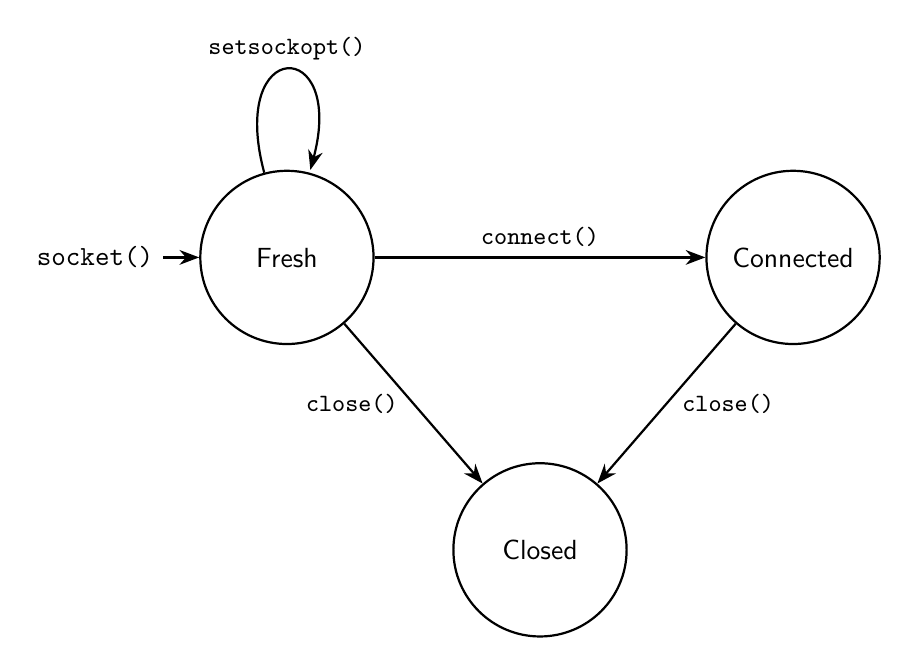
\begin{tikzpicture}[
    >={Stealth[length=2.5mm]},
    node distance=4.2cm,
    every state/.style={minimum size=22mm, thick, font=\sffamily},
    every edge/.style={draw, thick},
    lbl/.style={font=\ttfamily\small},
  ]
  \node[state, initial, initial text={\ttfamily socket()}] (fresh) {Fresh};
  \node[state, right=of fresh] (conn) {Connected};
  \node[state, below=2.6cm of $(fresh)!0.5!(conn)$] (closed) {Closed};

  \path[->]
    (fresh) edge[loop above] node[lbl, above] {setsockopt()} ()
    (fresh) edge node[lbl, above] {connect()} (conn)
    (fresh) edge node[lbl, left, xshift=-2pt] {close()} (closed)
    (conn)  edge node[lbl, right, xshift=2pt] {close()} (closed);
\end{tikzpicture}
\end{document}
